
\section{Pengembangan Prototipe \textit{High-Fidelity} Iterasi 1}
\label{sec:hifi_1}

Prototipe \textit{high-fidelity} adalah implementasi dari solusi desain yang dibuat sedekat mungkin dengan produk aslinya. Prototipe \textit{high-fidelity} memiliki fungsionalitas, elemen visual, dan interaksi yang lebih lengkap daripada prototipe \textit{low-fidelity}. \parencite{PreeceRogersSharp15} Prototipe yang dirancang mengembangkan seluruh tampilan pada Tabel \ref{tab:daftar_lofi_halaman} dan Tabel \ref{tab:daftar_lofi_widget} di bagian \ref{sec:lofi} pengembangan prototipe \textit{low-fidelity}, serta menerapkan lebih banyak prinsip desain sesuai yang telah disebutkan pada bagian \ref{tab:prinsip_desain}. Tujuan dari perancangan prototipe \textit{high-fidelity} ini adalah untuk mencapai \textit{usability goals} dan \textit{user experience goals} yang telah diharapkan dari analisis pada bagian \ref{subsec:analisis_goals}. Sebelum membuat prototipe, perlu ditentukan batasan implementasi, aspek antarmuka pengguna, serta komponen desain.


\subsection{Aspek Antarmuka Pengguna}
\label{subsec:antarmuka}

Secara umum, aspek-aspek antarmuka yang digunakan pada prototipe \textit{high-fidelity} ini mengacu pada sistem desain Material Design yang dibuat oleh Google. Panduan lengkap tentang Material Design dapat dilihat pada websitenya (\href{https://material.io/design}{https://material.io/design}). Material Design dipilih karena prototipe \textit{high-fidelity} ini merupakan perbaikan yang dilakukan untuk aplikasi Digital Wellbeing yang dibuat oleh Google. Aspek-aspek yang dipilih dari Material Design juga melihat aspek-aspek antarmuka dari aplikasi Digital Wellbeing awal. Berikut adalah penjelasan-penjelasan untuk setiap aspek antarmuka pada prototipe \textit{high-fidelity}  

\subsubsection{Warna}
\label{subsubsec:aspek_warna}
Warna yang digunakan dalam prototipe terbagi menjadi 3 kategori, yaitu warna primer, warna sekunder, dan warna aksen. Warna primer aplikasi menggunakan warna hijau, dengan alasan karena warna ini merupakan warna primer pada aplikasi Digital Wellbeing pada awalnya. Warna sekunder aplikasi adalah variasi atau gradasi warna monokrom hitam-putih. Selain itu, ada juga warna aksen yaitu warna kuning dan warna biru, yang juga sudah terdapat pada aplikasi Digital Wellbeing pada awalnya. Palet warna yang digunakan di aplikasi dapat dilihat pada Gambar \ref{img:pallete}.


\begin{figure}[h]
  \centering
  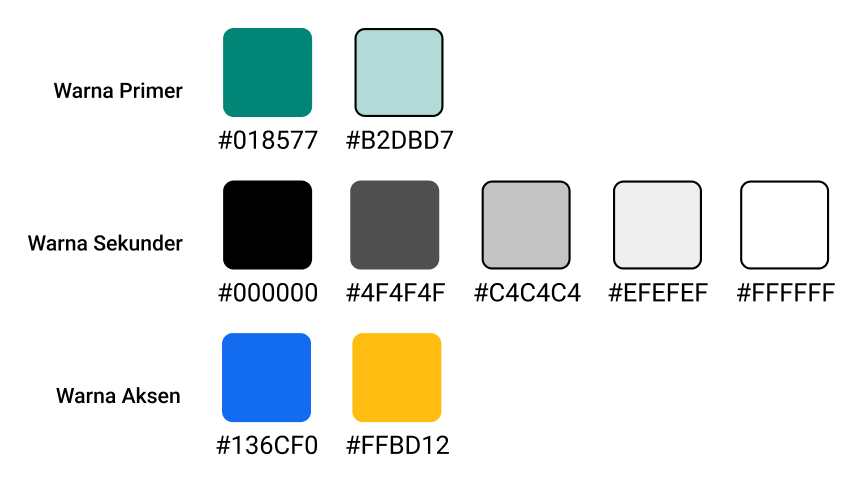
\includegraphics[width=0.7\textwidth]{chapter-4-color.png}
  \caption{Palet Warna Prototipe Aplikasi}
  \label{img:pallete}
\end{figure}
\FloatBarrier

\subsubsection{Tipografi}
\label{subsubsec:aspek_tipografi}
\textit{Typeface} yang digunakan dalam prototipe adalah Roboto, sesuai dengan \textit{typeface} yang digunakan oleh aplikasi Digital Wellbeing, dan merupakan \textit{typeface} standar yang digunakan dalam \textit{smartphone} berbasis Android.

\begin{figure}[h]
  \centering
  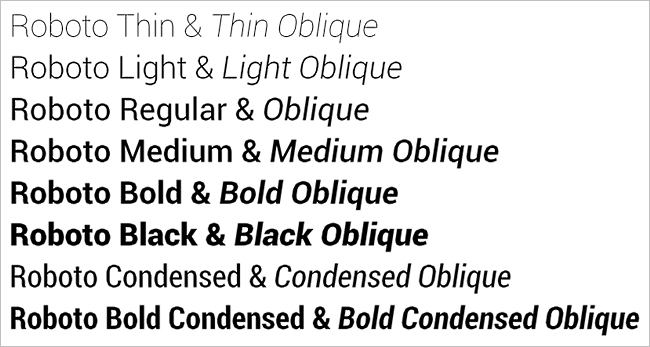
\includegraphics[width=0.6\textwidth]{chapter-4-roboto.jpg}
  \caption{\textit{Typeface} Roboto}
  \label{img:typeface}
\end{figure}
\FloatBarrier

\subsubsection{Ikon}
\label{subsubsec:aspek_ikon}
Ikon adalah simbol grafis yang dapat merepresentasikan sebuah fungsi atau objek pada antarmuka aplikasi. Penggunaan ikon yang sering ditemukan di tampilan aplikasi lain juga dapat memberikan rasa familiaritas, mempermudah fungsi-fungsi untuk dipelajari. Ikon-ikon yang digunakan pada prototipe \textit{high-fidelity} akan diambil dari ikon-ikon Material Design. Warna ikon akan mengikuti konteks dari antarmuka di sekelilingnya atau kondisi penggunaan tertentu, yaitu bisa menggunakan warna primer, sekunder, atau aksen. Ikon-ikon yang digunakan pada prototipe dapat ditemukan pada Gambar \ref{img:icons}

\begin{figure}[h]
  \centering
  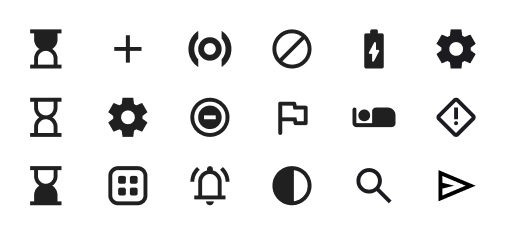
\includegraphics[width=0.5\textwidth]{chapter-4-icons.png}
  \caption{Ikon yang digunakan}
  \label{img:icons}
\end{figure}
\FloatBarrier
 
\subsubsection{Komponen Desain}
\label{subsubsec:komponen_hifi_1}

Berikut ini disebutkan beberapa komponen desain yang sering digunakan pada prototipe \textit{high-fidelity} Digital Wellbeing

\begin{enumerate}
  \item \textit{Button}
  \subitem Terdapat 3 jenis utama tombol pada prototipe, \textit{filled button}, \textit{border button}, dan \textit{text button}. Adapun variasi terhadap ukuran dan bentuk dari tombol yang diturunkan ketiga jenis utama. Tombol-tombol ini berperan penting dalam melakukan aksi dan menetapkan pengaturan. Beberapa tampilan memiliki deretan tombol-tombol jika terdapat lebih dari 1 aksi yang dapat dilakukan, maka dari itu desain yang berbeda dari tombol cukup penting untuk menegaskan hierarki kepentingan dari setiap aksi.
    \begin{figure}[h]
      \centering
      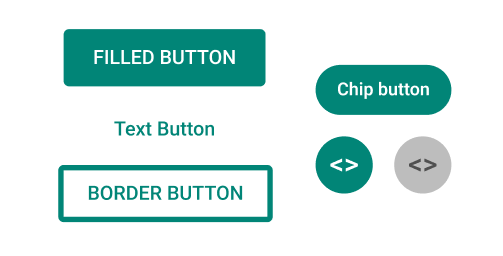
\includegraphics[width=0.45\textwidth]{chapter-4-buttons.png}
      \caption{Komponen \textit{button}}
      \label{img:button}
    \end{figure}
    \FloatBarrier
  
  \item Dialog
  \subitem Dialog adalah sebuah jendela kecil melayang yang digunakan untuk menampilkan secuplik informasi, meminta aksi dari pengguna, atau memuat pengaturan suatu fitur. Dialog sering dimanfaatkan pada prototipe untuk memuat pengaturan yang lebih kompleks atau informasi lebih di saat layar sudah cukup terpenuhi, berguna agar membebankan pengguna dengan tampilan yang terlalu rumit.

  \begin{figure}[h]
    \centering
    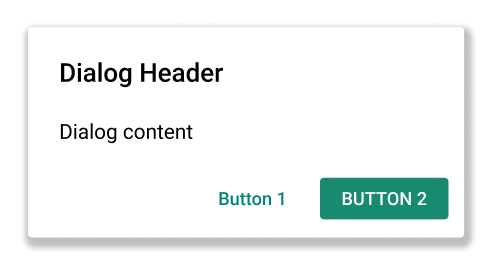
\includegraphics[width=0.4\textwidth]{chapter-4-dialog.png}
    \caption{Komponen dialog}
    \label{img:dialog}
  \end{figure}
  \FloatBarrier

  \item \textit{Time Picker}
  \subitem \textit{Time Picker} adalah sebuah variasi dari dialog yang berguna untuk memilih waktu. \textit{Time Picker} sering dimanfaatkan dalam prototipe, seperti untuk mengatur jadwal aktivasi Focus Mode atau App Timer.
  
  \begin{figure}[h]
    \centering
    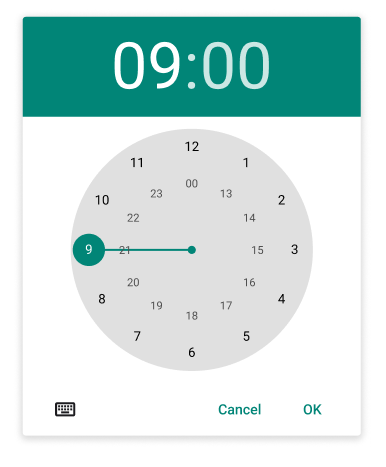
\includegraphics[width=0.35\textwidth]{chapter-4-timepicker.png}
    \caption{Komponen \textit{time picker}}
    \label{img:timepicker}
  \end{figure}
  \FloatBarrier

  \item \textit{Search bar}
  \subitem \textit{Search bar} adalah sebuah komponen untuk mencari sebuah benda dari dalam daftar. \textit{Search bar} sering dimanfaatkan pada prototipe karena banyaknya tampilan yang memuat daftar aplikasi, sehingga dibutuhkan untuk mempermudah pencarian aplikasi oleh pengguna.
 
  \begin{figure}[h]
    \centering
    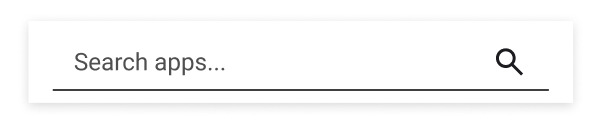
\includegraphics[width=0.6\textwidth]{chapter-4-seachbar.png}
    \caption{Komponen \textit{search bar}}
    \label{img:searchbar}
  \end{figure}
  \FloatBarrier

  \item \textit{Bar chart}
  \subitem \textit{Bar chart} atau diagram batang adalah sebuah grafik yang terusun dari kolom-kolom berbentuk batang. \textit{Bar chart} digunakan dalam prototipe untuk menyampaikan informasi tentang data penggunaan \textit{smartphone} atau aplikasi.
 
  \begin{figure}[h]
    \centering
    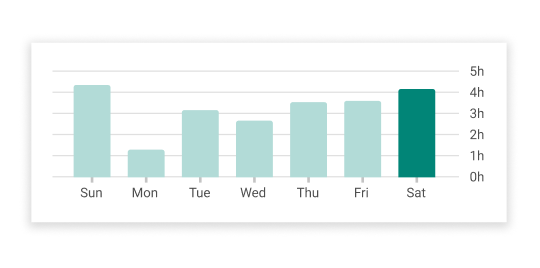
\includegraphics[width=0.5\textwidth]{chapter-4-barchart.png}
    \caption{Komponen \textit{bar chart}}
    \label{img:searchbar}
  \end{figure}
  \FloatBarrier

  \item \textit{Dropdown}
  \subitem \textit{Dropdown} adalah sebuah komponen desain yang berguna untuk mengelompokkan dan menyembunyikan objek-objek dengan atribut yang serupa. Komponen \textit{dropdown} dimanfaatkan pada prototipe untuk mengumpulkan pengaturan yang mirip pada suatu halaman, dan berguna untuk mengurangi beban visual dari tammpilan layar. Komponen \textit{dropdown} juga sudah digunakan pada aplikasi Digital Wellbeing pada awalnya.
 
  \begin{figure}[h]
    \centering
    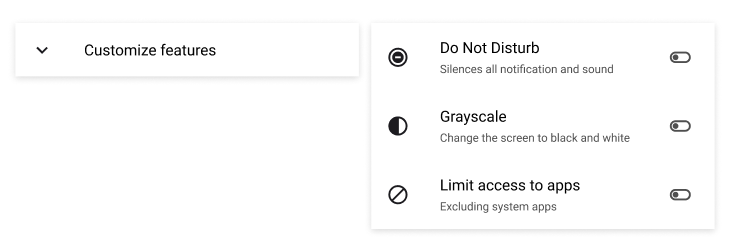
\includegraphics[width=0.6\textwidth]{chapter-4-dropdown.png}
    \caption{Komponen \textit{dropdown}}
    \label{img:dropdown}
  \end{figure}
  \FloatBarrier

\end{enumerate}


\subsection{Batasan Pengembangan}
\label{subsec:batasan_hifi_1}

Pengembangan prototipe \textit{high-fidelity} ini memiliki beberapa batasan agar pengembangan dapat fokus pada tujuan pengujian. Batasan-batasan pengembangan prototipe \textit{high-fidelity} adalah sebagai berikut

\begin{enumerate}
  \item Pengembangan prototipe \textit{high-fidelity} akan menggunakan \textit{prototyping tool} Figma.
  \item Data yang digunakan dalam prototipe berupa \textit{mock data} yang ditentukan oleh desainer.
  \item Prototipe dikembangkan untuk \textit{smartphone} berdimensi layar ukuran 360x800 pixel.
  \item Prototipe tidak mendukung kemampuan untuk input data kustom, bila komponen prototipe ditujukan untuk input data maka data yang ditunjukkan telah ditentukan oleh desainer.
  \item Tampilan prototipe menggunakan Bahasa Inggris. 
  \item Fitur rekomendasi pada prototipe tidak menggunakan rekomendasi nyata atas analisis data pengguna.
  \item Homescreen pada prototipe tidak mengacu pada tampilan \textit{smartphone} merk tertentu dengan alasan fokus pada tujuan untuk menguji komponen-komponen prototipe yang tidak dapat diakses dari dalam aplikasi.
\end{enumerate}

\subsection{Implementasi Prototipe \textit{High-Fidelity}}

Berdasarkan rencana perbaikan pada Tabel \ref{tab:daftar_perbaikan_lofi}, analisis aspek antarmuka, dan batasan pengembangan, maka tampilan-tampilan prototipe \textit{low-fidelity} pada Tabel \ref{tab:daftar_lofi_halaman} dan Tabel \ref{tab:daftar_lofi_widget} akan dikembangkan dan diimplementasi menjadi prototipe \textit{high-fidelity}. Tabel \ref{tab:daftar_hifi_halaman} memuat implementasi tampilan halaman prototipe \textit{high-fidelity}, sedangkan Tabel \ref{tab:daftar_hifi_widget} memuat implementasi tampilan untuk widget. Pada kedua tabel tersebut dimuat juga pemetaan prinsip desain tambahan terhadap prototipe \textit{high-fidelity}, serta penjelasan singkat tentang tampilan dan perubahannya dari tampilan prototipe \textit{low-fidelity}.


\newlength{\hifiwidth}
\setlength{\hifiwidth}{0.325\textwidth}

\newcommand{\hifi}[1]{\begin{center}\includegraphics[width=\hifiwidth]{#1}\end{center}}
\newcommand{\hifiwidget}[2]{\begin{center}\includegraphics[width=#1]{#2}\end{center}}

\RaggedLeft
\begin{footnotesize}
\begin{longtable}[c]{|>{\ccnormspacingcenter}p{0.12\textwidth}|>{\ccnormspacing}p{0.33\textwidth}|>{\ccnormspacingcenter}p{0.12\textwidth}|>{\ccnormspacingcenter}p{\hifiwidth}|}
  \caption{Daftar Tampilan Halaman Prototipe \textit{High-Fidelity}}
  \label{tab:daftar_hifi_halaman} \\
  \hline \rowcolor[HTML]{A3E5F5}
  \centering\textbf{Halaman} & \centering\textbf{Penjelasan Halaman} & \centering\textbf{Prinsip Desain Tambahan} & \textbf{Prototipe \textit{High-Fidelity}} \\ \hline \endfirsthead
  \hline \rowcolor[HTML]{A3E5F5}
  \centering\textbf{Halaman} & \centering\textbf{Penjelasan Halaman} & \centering\textbf{Prinsip Desain Tambahan} & \textbf{Prototipe \textit{High-Fidelity}} \\ \hline \endhead
  \hline \endfoot

  \textbf{H-01} Halaman Main Menu & Halaman ini adalah tampilan utama dari aplikasi Digital Wellbeing yang memuat navigasi utama ke fitur-fitur lainnya. Pada prototipe \textit{high-fidelity} terdapat perubahan pada bentuk menu navigasi menjadi lebih bundar agar lebih \textit{user-friendly}. Adapun implementasi ilustrasi untuk menu Focus Mode dan Bedtime Mode, dan ikon-ikon pada menu lainnya, menggantikan \textit{placeholder} pada tampilan \textit{low-fidelity}. & - & \hifi{hifi/h-01} \\ \hline
  
  \textbf{H-02} Halaman Dashboard & Halaman ini memuat seluruh data penggunaan \textit{smartphone}. Pada prototipe \textit{high-fidelity} terdapat penambahan warna untuk \textit{bar chart} agar memperjelas data yang sedang dipilih. Adapun pengubahan desain dari tombol penambahan App Group untuk memberikan perbedaan yang jelas dengan tombol navigasi ke halaman data penggunaan App Group & - & \hifi{hifi/h-02} \\ \hline
  
  \textbf{H-03} Halaman App Timer & Halaman ini berisi daftar App Timer yang telah dipasang oleh pengguna, dan daftar aplikasi lain. Pada prototipe \textit{high-fidelity}, menu konfigurasi pengingat App Timer disembunyikan di dalam komponen \textit{dropdown} untuk mengurangi kompleksitas visual. Selain itu, ada juga penambahan bagian yang memuat daftar App Group yang sudah dibuat, memindahkan lokasi App Group dari dalam daftar aplikasi. & - & \hifi{hifi/h-03} \\ \hline
  
  \textbf{H-04} Halaman Daily Goal & Di halaman ini, pengguna dapat menentukan Daily Goal atau tujuan harian yang ingin ditempuh dan dibantu diingatkan oleh aplikasi Digital Wellbeing. Pada prototipe \textit{high-fidelity} terdapat penambahan penjelasan untuk fitur-fitur pengingat Daily Goal agar lebih mudah untuk dimengerti. Adapun penambahan ikon untuk fitur Daily Goal agar tampilan tidak terasa kaku & - & \hifi{hifi/h-04} \\ \hline
  
  \textbf{H-05} Halaman Focus Mode & Halaman ini memuat status dari keberjalanan Focus Mode serta aksi-aksi yang dapat dilakukan untuk menunda, mematikan, atau mengaktivasinya. Pada prototipe \textit{high-fidelity} terdapat penambahan daftar aplikasi untuk memilih aplikasi yang dinilai mendistraksi, daftar ini dapat dimanfaatkan jika pengguna ingin menyalakan fitur Focus Mode tanpa mengikuti jadwal. Adapun pemindahan lokasi navigasi ke halaman penambahan jadwal Focus Mode agar lebih mudah diakses jika terdapat banyak jadwal Focus Mode. & - & \hifi{hifi/h-05} \\ \hline
  
  \textbf{H-06} Halaman Bedtime Mode &  Pada halaman ini, pengguna dapat mengatur jadwal aktivasi Bedtime Mode menurut mode perilaku aktivasi yang dipilihnya. Pada prototipe \textit{high-fidelity} terdapat penambahan penjelasan singkat tentang mode aktivasi While Charging, sesuai dengan rencana perbaikan terhadap masalah yang dilaporkan. Adapun penambahan warna aksen terhadap pengaturan jadwal, warna aksen ini sudah menjadi bagian dari aplikasi Digital Wellbeing pada awalnya. Selain itu, menu konfigurasi kemampuan yang aktif saat Bedtime Mode disembunyikan di dalam komponen \textit{dropdown} untuk mengurangi kompleksitas visual. & - & \hifi{hifi/h-06-schedule} \\ \hline
  
  \textbf{H-07} Halaman Ringkasan Penggunaan Aplikasi & Halaman ini memuat data penggunaan sebuah aplikasi. Pada prototipe \textit{high-fidelity}, terdapat penambahan ikon pada navigasi App Timer dan pengaturan notifikasi agar tampilan lebih mudah dikenali. & - & \hifi{hifi/h-07} \\ \hline
  
  \textbf{H-08} Halaman Ringkasan Penggunaan App Group & Halaman ini memuat data penggunaan dari App Group atau kelompok aplikasi yang ditentukan oleh pengguna. Pada prototipe \textit{high-fidelity}, terdapat penambahan ikon pada navigasi App Timer dan pengaturan App Group agar tampilan lebih mudah dikenali. & - & \hifi{hifi/h-08} \\ \hline
  
  \textbf{H-09} Halaman Pengaturan App Group & Pada halaman ini dapat dilakukan pengaturan terhadap App Group yang dibuat oleh pengguna. Pada prototipe \textit{high-fidelity}, tidak ada perubahan yang cukup signifikan selain pengaplikasian warna. & - & \hifi{hifi/h-09} \\ \hline
  
  \textbf{H-10} Halaman Pengaturan Jadwal App Timer & Pada halaman ini dapat dilakukan pengaturan terhadap App Timer aplikasi yang dibuat oleh pengguna. Pada prototipe \textit{high-fidelity} terdapat perubahan tampilan untuk pengaturan App Timer, dengan memberikan elemen untuk mengkonfirmasi pengaturan sesuai dengan rancangan perbaikan dari prototipe \textit{low-fidelity}. Adapun jika belum ada opsi mode aktivasi App Timer, maka tombol konfirmasi pengaturan akan dinonaktifkan. & DP-07 & \hifi{hifi/h-10-daily} \hifi{hifi/h-10-off} \\ \hline
  
  \textbf{H-11} Halaman Pengaturan Jadwal Focus Mode & Pada halaman ini, pengguna dapat mengatur hari dan waktu aktivasi dari jadwal Focus Mode yang dibuat pengguna. Pada prototipe \textit{high-fidelity} terdapat penambahan bagian yang memuat daftar App Group yang sudah dibuat, memindahkan lokasi App Group dari dalam daftar aplikasi, agar pengguna lebih mudah dalam memilih sekelompok aplikasi sekaligus. & - & \hifi{hifi/h-11} \\ \hline
  
  \textbf{H-12} Halaman Pengenalan Dashboard & Halaman ini memuat ilustrasi tujuan dari Dashboard dan penjelasan tentang fitur-fitur yang terdapat pada Dashboard. Pada prototipe \textit{high-fidelity} dilakukan perubahan ukuran \textit{font} dari deskripsi agar lebih mudah dibaca. Adapun penambahan ilustrasi agar fitur-fitur yang dijelaskan lebih mudah untuk dipelajari. & - & \hifi{hifi/h-12} \\ \hline
  
  \textbf{H-13} Halaman Pengenalan App Timer & Halaman ini memuat ilustrasi tujuan dari App Timer dan penjelasan tentang fitur-fitur yang terdapat pada App Timer. Pada prototipe \textit{high-fidelity} dilakukan perubahan ukuran \textit{font} dari deskripsi agar lebih mudah dibaca. Adapun penambahan ilustrasi agar fitur-fitur yang dijelaskan lebih mudah untuk dipelajari. & - & \hifi{hifi/h-13} \\ \hline
  
  \textbf{H-14} Halaman Pengenalan Goal Reminder & Halaman ini memuat ilustrasi tujuan dari Goal Reminder dan penjelasan tentang fitur-fitur yang terdapat pada Goal Reminder. Pada prototipe \textit{high-fidelity} dilakukan perubahan ukuran \textit{font} dari deskripsi agar lebih mudah dibaca. Adapun penambahan ilustrasi agar fitur-fitur yang dijelaskan lebih mudah untuk dipelajari. & - & \hifi{hifi/h-14} \\ \hline
  
  \textbf{H-15} Halaman Pengenalan Focus Mode & Halaman ini memuat ilustrasi tujuan dari Focus Mode dan penjelasan tentang fitur-fitur yang terdapat pada Focus Mode. Pada prototipe \textit{high-fidelity} dilakukan perubahan ukuran \textit{font} dari deskripsi agar lebih mudah dibaca. Adapun penambahan ilustrasi agar fitur-fitur yang dijelaskan lebih mudah untuk dipelajari. & - & \hifi{hifi/h-15} \\ \hline
  
  \textbf{H-16} Halaman Pengenalan Bedtime Mode & Halaman ini memuat ilustrasi tujuan dari Bedtime Mode dan penjelasan tentang fitur-fitur yang terdapat pada Bedtime Mode. Pada prototipe \textit{high-fidelity} dilakukan perubahan ukuran \textit{font} dari deskripsi agar lebih mudah dibaca. Adapun penambahan ilustrasi agar fitur-fitur yang dijelaskan lebih mudah untuk dipelajari. & - & \hifi{hifi/h-16} \\ \hline

\end{longtable}
\end{footnotesize}
\justifying
\FloatBarrier

\RaggedLeft
\begin{footnotesize}
\begin{longtable}[c]{|>{\ccnormspacingcenter}p{0.08\textwidth}|>{\ccnormspacing}p{0.37\textwidth}|>{\ccnormspacingcenter}p{0.1\textwidth}|>{\ccnormspacingcenter}p{\lofiwidth}|}
  \caption{Daftar Tampilan Widget Prototipe \textit{High-Fidelity}}
  \label{tab:daftar_hifi_widget} \\
  \hline \rowcolor[HTML]{A3E5F5}
  \centering\textbf{ID Widget} & \centering\textbf{Penjelasan Widget} & \centering\textbf{Prinsip Desain} & \textbf{Prototipe \textit{Low-Fidelity}} \\ \hline \endfirsthead
  \hline \rowcolor[HTML]{A3E5F5}
  \centering\textbf{ID Widget} & \centering\textbf{Penjelasan Widget} & \centering\textbf{Prinsip Desain} & \textbf{Prototipe \textit{Low-Fidelity}} \\ \hline \endhead
  \hline \endfoot
  
  \textbf{W-01} Widget Dashboard & Widget ini memuat data penggunaan \textit{smartphone}, serta 3 aplikasi dengan penggunaan tertinggi pada hari tersebut. Desain widget pada prototipe \textit{high-fidelity} dibuat menjadi lebih \textit{user-friendly} agar widget dapat lebih berbaur dengan tampilan pada Homescreen.  & - & \hifiwidget{0.2\textwidth}{hifi/w-01} \\ \hline

  \textbf{W-02} Widget App Timer & Widget ini memuat daftar aplikasi yang telah dipasang App Timer, serta sisa waktu untuk menggunakan aplikasi sebelum aksesnya ditutup. Desain widget pada prototipe \textit{high-fidelity} dibuat menjadi lebih \textit{user-friendly} agar widget dapat lebih berbaur dengan tampilan pada Homescreen.  & - & \hifiwidget{0.325\textwidth}{hifi/w-02} \\ \hline
  
  \textbf{W-03} Widget Focus Mode & Widget ini menampilkan status keberlangsungan dari Focus Mode. Desain widget pada prototipe \textit{high-fidelity} dibuat menjadi lebih \textit{user-friendly} agar widget dapat lebih berbaur dengan tampilan pada Homescreen. Ada juga penambahan interaksi pada widget agar pengguna dapat memanfaatkan lebih banyak fungsionalitas dari Focus Mode. & - & \hifiwidget{0.325\textwidth}{hifi/w-03} \\ \hline

\end{longtable}
\end{footnotesize}
\justifying
\FloatBarrier

